\documentclass[a4paper,11pt, twoside]{article}
%\usepackage[firstpage]{draftwatermark}
%\SetWatermarkLightness{0.5}
%\SetWatermarkScale{4}
\setcounter{tocdepth}{2}
\usepackage[dutch]{babel}
\usepackage{xspace, color, mdframed}
\usepackage[usenames,dvipsnames]{xcolor}
\usepackage{graphicx,listings,float,epstopdf,geometry,amsmath,placeins,caption,subcaption,placeins,pdfpages}

\geometry{
	includeheadfoot,
	margin=2.54cm
}

% Commando abstract
\addto\captionsdutch{\renewcommand*\abstractname{Abstract}}

% Commando's werkplan
\newcommand{\BS}{BrnStrm}
\newcommand{\ON}{Ori\"entatie}
\newcommand{\MW}{Werkplan}
\newcommand{\MS}{SpelSpec}
\newcommand{\MA}{Spelkeus}
\newcommand{\BO}{Deel. Docu.}
\newcommand{\OC}{Protocol}
\newcommand{\MN}{Impl.Proto.}
\newcommand{\CT}{Proto Test}
\newcommand{\MK}{Klas.diagr.}
\newcommand{\MT}{Taakverdel.}
\newcommand{\IS}{Implement}
\newcommand{\BG}{Handl.}
\newcommand{\AV}{Eind Docu}
\newcommand{\ME}{Mkn.prsnt.}
\newcommand{\EP}{Presenteren}

% Commando's ontwerp
\newcommand{\protoref}{sectie \ref{sec:protocol}}

\newcommand{\bericht}[1]{
    {\begin{center}
        \colorbox{YellowGreen!20}{\makebox[\textwidth][c]{{
            \textsc{#1}
        }}}
    \end{center}
}}

\newcommand{\udp}{\textsc{udp}\xspace}
\newcommand{\tcp}{\textsc{tcp}\xspace}

% Server
% Lobby
\begin{document}
	\input{title}

	\tableofcontents
	\newpage

	\section{Lijst symbolen en afkortingen}
    % Verklaring van alle gebruikte symbolen
        De volgende tabel bevat alle gebruikte symbolen en afkortingen in dit verslag:
    \begin{table}[H]
        \small
        \centering
        \begin{tabular}{| l | l |}
        \hline
        Symbool / Afkorting & Verklaring \\ \hline
        GOTO & Grudge of the Oblivious, de naam voor ons spel \\ \hline
        $\sigma$ & Symbool voor een permutatie \\ \hline
        $<$ & Symbool voor een totale ordening \\ \hline
        $\langle\langle \rangle\rangle$ & Symbool voor het implementeren van een interface \\ \hline
        OGO & Ontwerp Gericht Onderwijs \\ \hline
        UML & Unified Modeling Language \\ \hline
        MSC & Message Sequence Chart \\ \hline
        GUI & Graphical User Interface \\ \hline
        3D & Driedimensionaal \\ \hline
        LAN & Local area network \\ \hline
        FPS & First-Person Shooter \\ \hline
        RTS & Real-Time Strategy \\ \hline
        BNF & Backus-Naur Form \\ \hline
        TCP & Transmission Control Protocol \\ \hline
        UDP & User Datagram Protocol \\ \hline
        RTT & Round-Trip Time \\ \hline
        FIFO & First In, First Out \\ \hline
        ID & Identifier \\ \hline
        TID & Team identifier \\ \hline
        PID & Player identifier \\ \hline
        CIDR & Classless Inter-Domain Routing \\ \hline
        IP & Internet Protocol \\ \hline
        Mbps & Megabit per seconde \\ \hline
        CD-ROM & Compact Disc Read-only memory \\ \hline
        \end{tabular}
        \caption{Symbolen en afkortingen in het eindverslag}
        \label{tab:planning}
    \end{table} 	
    \newpage

    \section{Summary}
    % Engelstalige samenvatting
    \emph{Grudge of the Oblivious} (\textsc{goto}) is a multiplayer 3D game. It combines elements of First-Person Shooters and Real-Time Strategy. Two robot gangs fight for world domination. Every player has its own robot to fight for one of these gangs. The goal of the game is to destroy the headquarter of the opposing gang. Players can attack the headquarter by shooting with their powerful laser guns.

    In order to defend their own headquarter, players can attack other players by shooting with their laser guns, which weakens their armor. When the armor of a player is fully destroyed, the player will return to the game with new armor at its headquarter after a small time period. Players can also defend their headquarter by building defense towers with gold. When a player of the opposing team is near such a defense tower, the defense tower will attack the player.

    Gold can be earned in two ways. Firstly, gold can be earned by building mines over mining spots. Alternatively, gold can be earned by killing opposing players or destroying opposing buildings. When an opposing player is killed or an opposing building is destroyed, a coin will be dropped on the ground. This coin can be picked up by all other players.

    The game was developed for the \textsc{ogo} 2.3 project. This document contains the documentation for the various steps taken in the development. We started our development of the game by studying the different challenges. We note that our game can be played over a \textsc{lan} or over the Internet. Mutual exclusion is thus required to keep the game in a consistent state. It is for example not desirable that two players can pick up the same coin. Therefore, a communication protocol needs to be developed that enforces mutual exclusion.

    The three most difficult challenges were the networking, mutual exclusion and complexity in our opinion. With complexity we mean the challenges associated with large programs. After identifying the most critical challenges we were able to give a tight time schedule for the development. We were then able to give a specification of the game. Here we also considered various alternatives. We will explore these alternatives and explain our choices.

    Having specified the game, we were then ready to do a thorough analysis of the game design. The different components were identified: the protocol, the \textsc{gui} and the scene model. We will describe these components and study the relationship between them. Next we turn our attention to the protocol. We formally define a message format and the different messages used for communication. We will also discuss the working of the protocol.
    Mutual exclusion in the protocol was implemented using a token ring. Since the protocol is highly complex, several test programs have been developed. Special attention was paid in order to identify and validate the underlying assumptions in the protocol. We will motivate our choices during the implementation. We end by giving a conclusion and an evaluation.
    \newpage

    \section{Inleiding}
    % Probleem- of vraagstelling
    % Opbouw
    Informatici in de hedendaagse wereld komen vaak in aanraking met het ontwerpen van complexe programma's. Complexe programma's hebben vaak ook een netwerk aspect en een grafische aspect. Zelfs bij technische programma's, die vaak minder grafisch intensief zijn, zijn deze aspecten al vaak belangrijk. Dit geeft duidelijk de noodzaak aan dat elke informaticus kennis heeft van computergrafiek, computernetwerken en het ontwerpen van complexe programma's. Al deze aspecten worden verenigd in dit project: \textsc{ogo} 2.3 - Nethunt.

Voor dit project werd ons gevraagd om een interactief, gedistribueerd 3D-spel te ontwikkelen. Dit spel moest over een \textsc{lan} kunnen worden gespeeld. Wij hebben ervoor gekozen om spelers ook de mogelijkheid te geven om over het internet te spelen. Een eis bij de implementatie was een vorm van symmetrie tussen de verschillende spelers. Hier bedoelen we mee dat elke speler lokaal dezelfde spelsituatie heeft. Bovendien staan de verschillende spelers op gelijke voet gedurende het spel. Er mag dus geen server aanwezig zijn tijdens het spel. Een andere eis was dat er een vorm van voedsel aanwezig moet zijn. We willen niet dat verschillende spelers hetzelfde voedsel kunnen oppakken, dus er is een vorm van mutual exclusion vereist.

Dit document bevat de documentatie voor dit project. We zullen beginnen door een strakke planning te geven in de vorm van een werkplan. Daarna gaan we verder met een specificatie van het spel. Hierbij beschrijven we ook de alternatieven en de motivering voor onze keuze. We zijn dan klaar om een ontwerp van het spel te geven, inclusief het communicatieprotocol. De impliciete aannamen in het communicatieprotocol zullen we proberen te identificeren. We sluiten af met een validatie van deze aannamen en een motivering voor de implementatie, gevolgd door een conclusie en evaluatie. In de appendices is nog verdere documentatie opgenomen. Voor het lezen van het document kan het nuttig zijn om appendix \ref{app:begrippen} te bestuderen, waar een volledige begrippenlijst is opgenomen.

Bij de implementatie hebben we gebruik gemaakt van \emph{Doxygen}. Dit programma genereert automatisch documentatie op basis van commentaar in de code en de algemene structuur. Deze documentatie is apart toegevoegd op de \textsc{cd-rom} als Doxygen.pdf. 

    \input{werkplan}
        \section{Specificatie}
    Het spel, \emph{Grudge of the Oblivious} (\textsc{goto}), dat wij van plan zijn om te ontwerpen, is een combinatie van een FPS spel en een RTS spel. Dit betekent dat de gebruiker van het spel zowel kan schieten als gebouwen kan bouwen. We beschrijven in appendix \ref{app:alternatieven} de door ons geanalyseerde alternatieve ontwerpen voor een spel. In appendix \ref{app:motivering} motiveren wij de keuze voor ons spel. Op basis van deze specificatie is er een gebruikershandleiding gemaakt. De gebruikershandleiding is te vinden in appendix \ref{app:handleiding}.

    Het spel speelt zich af in een oorlog tussen twee rivaliserende robot-bendes. Deze robot-bendes hebben een corresponderend commandocentrum. In het spel kan een robot-bende als team gezien worden, een dergelijk team bestaat uit meerdere robots en spelers. Elke speler bestuurt \'e\'en robot. Er zijn evenveel robots als spelers.

    Het doel van het spel is om het commandocentrum van de tegenstander te vernietigen. De spelers hebben lasergeweren om de tegenstanders dood te schieten en torens aan te vallen. Torens kunnen door spelers worden neergezet op het terrein. Deze torens kosten goud om te bouwen. De spelers verdienen goud in een gezamenlijke kas door mijnen te bouwen over delfplaatsen. Verder kan goud worden verdiend door tegenstanders te doden en hun torens te vernietigen. Als een speler dood gaat of een toren kapot gaat, zal deze een muntje achterlaten dat vervolgens door alle spelers kan worden opgepakt. Wij richten ons met dit spel voornamelijk op jongeren van 14 tot 25 jaar.

    Hier beschrijven we alleen de noodzakelijke onderdelen van het spel. Een lijst van mogelijke uitbreidingen is toegevoegd in appendix \ref{app:optioneel}.

	\subsection{Terrein}
    Het terrein kan in wezen allerlei vormen hebben, we leggen hier slechts twee simpele restricties op. Allereerst moet het terrein eerlijk zijn: dit betekent dat een team geen voordeel mag hebben vanwege de kaart. We eisen bovendien dat de kaart rechthoekig is.

    Op het terrein zijn twee commandocentra geplaatst, voor beide teams een commandocentrum. Het kan gewenst zijn dat elk team bij de start van het spel ook al een aantal extra torens heeft ter bescherming van het commandocentrum. Over het terrein zijn een aantal delfplaatsen verdeeld. Andere obstakels mogen aanwezig zijn, maar zijn niet noodzakelijkerwijs aanwezig. Alle objecten met uitzondering van spelers worden geplaatst op een rooster. In figuur \ref{fig:map1} en \ref{fig:map2} zijn twee mogelijke beginconfiguraties van het spel getoond.

    \begin{figure}[h]
        \begin{subfigure}{0.5\linewidth}
            \includegraphics[width=\textwidth]{../Graphics/Map1.eps}
            \caption{Een bijna vierkant terrein met vier spelers}
            \label{fig:map1}
        \end{subfigure}\hspace{10mm}
        \begin{subfigure}{0.5\textwidth}
                \includegraphics[width=\textwidth]{../Graphics/Map2.eps}
                \caption{Een breed terrein met drie spelers}
                \label{fig:map2}
        \end{subfigure}
        \caption{Twee verschillende beginconfiguraties van het spel}
    \end{figure}

    \subsection{Spelers}
    Een speler behoort tot \'e\'en van beide teams, spelers van een bepaald team zijn te identificeren door kleuren. De speler ziet de wereld vanuit de positie van zijn robot. Men kan de kijkrichting aanpassen, zodat deze elke willekeurige richting kan zijn. Als de kijkrichting verder naar links of rechts wordt gedraaid, draait de robot mee. De speler heeft een lasergeweer waarmee hij op andere spelers en torens kan schieten om deze te vernietigen. Het lasergeweer schiet laserstralen met een `oneindige' snelheid in de huidige kijkrichting. Bij het begin van het spel heeft de robot nog een volledig harnas. Zodra de speler wordt geraakt, wordt de conditie van het harnas slechter. 
    \FloatBarrier
    Een speler gaat dood als zijn harnas kapot is. In dat geval zal hij na een bepaalde hoeveelheid tijd terugkeren bij het commandocentrum met een volledig harnas. Ook kan een speler gebouwen bouwen, hiervoor gebruikt hij goud uit de kas van het team. De spelers kunnen op het grondvlak bewegen met een vaste snelheid in elke richting. De enige voorwaarde hierbij is dat de spelers op de kaart blijven en niet door een gebouw lopen. Het is dus wel mogelijk dat spelers door elkaar heen kunnen lopen. De speler kijkt vanuit een derde persoon perspectief. In een derde persoon perspectief wordt de sc\`ene bekeken vanaf een punt vlak achter de speler. Het is eventueel mogelijk om dit verder uit te breiden, zodat de speler kan wisselen van derde persoon perspectief naar eerste persoon perspectief.

    \subsection{Gebouwen}
    Er zijn drie soorten gebouwen: torens, mijnen en commandocentra. Torens schieten op spelers en andere gebouwen in hun bereik. Mijnen kunnen over delfplaatsen worden gebouwd met het doel de inkomsten van een team te vergroten. In principe levert elke mijn een vaste hoeveelheid goud voor de gezamenlijke kas op. Deze hoeveelheid wordt periodiek toegevoegd aan de kas.

    Uit sommige delfplaatsen kan maar een bepaalde hoeveelheid goud worden gehaald, daarna is de delfplaats op. Dan zal de mijn over die delfplaats geen verdere bijdrage meer leveren voor de gezamenlijke kas. We staan echter ook delfplaatsen toe die een onbeperkte hoeveelheid goud bevatten. Standaard levert elke mijn hetzelfde bedrag op met dezelfde periode, maar dit kan later nog worden aangepast.

    Het commandocentrum is het belangrijkste gebouw van het team. Als dit gebouw kapot is, heeft het bijbehorende team verloren. Gebouwen kunnen door spelers worden beschoten, waardoor deze worden beschadigd. Gebouwen kunnen op geen enkele mogelijke manier hersteld worden. Optioneel zou men mechanismen in het spel kunnen toevoegen om deze gebouwen te herstellen. Alle gebouwen behoren tot \'e\'en van beide teams, deze gebouwen kunnen weer ge\"identificeerd worden door de kleur van het gebouw.

    \subsection{Verzamelbare voorwerpen}
    Er is maar \'e\'en verzamelbaar voorwerp: een muntje. E\'en of meerdere muntjes worden achtergelaten door spelers die dood gaan en torens die worden vernietigd. Een muntje heeft een bepaalde waarde in goud. De waarde van de muntjes zijn proportioneel aan de gezamenlijke kas van het team waarvan de speler is doodgegaan. Als een toren is vernietigd, dan is de waarde van de muntjes proportioneel aan de kosten van de toren. De waarde van de muntjes moet echter altijd kleiner zijn dan de kosten van de toren. Gedurende een spel moeten deze proporties vast zijn.

    Als een speler doodgaat, wordt bovendien nog de waarde van de muntjes afgetrokken van de gezamenlijke kas van die speler. Een muntje kan vervolgens opgepakt worden door alle spelers. Het muntje is dus het voedsel element in ons spel. De waarde van het muntje zal dan toegevoegd worden aan de kas van het bijbehorende team.

    \subsection{Initialisatie}
    De spelers kunnen zelf kiezen bij welk team ze gaan, onder de voorwaarde dat elk team minstens \'e\'en speler heeft. Bij de start van het spel staan alle spelers bij het commandocentrum. Zoals al eerder gezegd, hebben alle spelers dan nog een volledig harnas. Bovendien heeft elk team een zekere positieve hoeveelheid goud in de gezamenlijke kas, die voor beide teams natuurlijk gelijk moet zijn. Er kan minstens \'e\'en mijn gebouwd worden met deze hoeveelheid goud.
    \FloatBarrier

    \subsection{Gebruikersomgeving}
    \label{sec:UI}

    Via de gebruikersomgeving kan de speler de interactie met het 3D-model aangaan. De volgende componenten worden weergegeven op de gebruikersomgeving tijdens het spel:
    \begin{itemize}
    \item De hoeveelheid goud van het team, deze hoeveelheid staat achter een goudstaaf.
    \item De sterkte van het harnas, die wordt weergegeven door middel van een statusbalk.
    \item Het vizier van de speler.
    \item Een plattegrond.
    \end{itemize}

    We plaatsen het vizier van de speler altijd in het midden van het scherm. Hierdoor weet de speler dus in welke richting wordt geschoten. Voor de duidelijkheid hebben wij hier ook een figuur van gemaakt, zie figuur \ref{fig:UI1}.
    \begin{figure}[H]
    \includegraphics[width=0.9\textwidth]{../Graphics/UI.eps}
    \caption{De gebruikersomgeving tijdens het spel}
    \label{fig:UI1}
    \end{figure}
    De besturing van de robot kan met de \textsc{wasd}-toetsencombinatie of door gebruik te maken van de pijltjes-toetsen. Hiervoor geven we de volgende tabel:
    \begin{table}[H]
        \small
        \centering
        \begin{tabular}{| l | l |}
        \hline
        Knop & Reactie \\ \hline
        \textsc{w} of $\uparrow$ & De robot beweegt, indien mogelijk, vooruit naar de huidige kijkrichting toe \\ \hline
        \textsc{a} of $\leftarrow$ & De robot draait naar links \\ \hline
        \textsc{s} of $\downarrow$ & De robot beweegt, indien mogelijk, achteruit van de huidige kijkrichting af \\ \hline
        \textsc{d} of $\rightarrow$ & De robot draait naar rechts \\ \hline
        \end{tabular}
        \caption{Knoppen met bijbehorende reactie}
        \label{tab:planning}
    \end{table}

    De speler kan schieten door op de muis te drukken. Een gedetailleerde beschrijving van het schieten is opgenomen in appendix \ref{app:schieten}. Door de muis naar boven of naar beneden te bewegen, kijkt de speler verder omhoog of omlaag respectievelijk. Op analoge wijze kan de speler naar links of naar rechts draaien door respectievelijk de muis naar links of naar rechts te bewegen. Merk op dat het vizier altijd in het midden van het scherm blijft. De speler ziet dit dus doordat de horizon omlaag of omhoog schuift.

    \subsection{Het neerzetten van gebouwen}
    De speler kan ook opdracht geven om op een bepaalde plek een gebouw neer te laten zetten. Om een gebouw neer te zetten moet de speler eerst op de knop \textsc{b} drukken. Dan gaat de speler in de zogenaamde \emph{bouw-modus}. Er wordt dan op de ondergrond een rooster getekend. Door middel van het vizier kan de speler een plek op het rooster aanwijzen. De speler kan dan door te klikken de opdracht geven om het gebouw te plaatsen. Op dat moment wordt de bijbehorende hoeveelheid goud uit de gezamenlijke kas gehaald. Dit kan natuurlijk alleen als de speler voldoende goud heeft.

    Indien de speler niet genoeg goud heeft, dan zal er een waarschuwing worden gegeven. Het gebouw zal dan ook niet worden geplaatst. Als de speler wel genoeg goud heeft, zal het gebouw uit de grond verrijzen. Na het neerzetten van het gebouw blijft de speler in de bouw-modus. Door nogmaals op de knop \textsc{b} te drukken gaat de speler weer uit de bouw-modus. Dit kan gezien worden in figuur \ref{fig:gebouw}.
    \begin{figure}
    \centering
    \includegraphics[width=\textwidth]{../Graphics/UI2.pdf}
    \caption{Een voorbeeld van het neerzetten van een gebouw in de gebruikersomgeving}
    \label{fig:gebouw}
    \end{figure} 
        \section{Het ontwerp}
    % Inclusief alternatieven, motivering van keuzes, aannames en communicatieprotocol
    Nu zijn we klaar om het ontwerp van ons spel \textsc{GOTO} te bespreken. We zullen beginnen door de verschillende componenten te analyseren. Het programma is hierbij verdeeld in drie zo onafhankelijk mogelijke componenten. Wij onderscheiden de volgende componenten:
    \begin{itemize}
    \item Een component die het communiceren naar andere spelers mogelijk maakt;
	\item Het model van de sc\`ene. Denk hierbij aan de staat, locatie en grafische modellen van gebouwen, spelers en het terrein;
	\item De gebruikersomgeving die de interactie van de speler met het spel mogelijk maakt en ook het grafische model weergeeft tijdens het spel.
    \end{itemize}

    Als uitgangspunt ontwerpen wij de verschillende componenten zodanig dat elke component zo onafhankelijk mogelijk ontwikkeld kan worden.
    	
    \subsection{Protocol module}
    De protocol module is het onderdeel die het mogelijk maakt om:
	\begin{itemize}
    \item Een nieuw spel op te starten. Het spel komt dan in de zogenaamde opstart fase. Andere spelers kunnen dan aan dit spel meedoen, ze komen dan in de lobby van dat spel. We hebben ervoor gekozen om de lobby te integreren in het spel;
	\item De lijst van alle spellen, die nog in de opstart fase zijn, in het subnet van de computer weer te geven;
	\item Mee te doen met een bestaand spel dat nog in de opstart fase zit;
	\item Het spel te beginnen;
	\item Mutaties van de staat van het spel te ontvangen en te versturen.
	\end{itemize}
    De manier, waarop deze communicatie verloopt, is beschreven vanaf \protoref. De gebruikersomgeving kan de protocol module een opdracht geven. Deze    opdracht zal dan asynchroon worden uitgevoerd door de protocol module. Dit betekent dat het protocol uit zichzelf berichten kan ontvangen en verwerken. Door middel van threads wordt er voor gezorgd dat het protocol de taken onafhankelijk kan uitvoeren.
	
    \subsection{Het model van de sc\`ene}
    Het model van de sc\`ene vervult twee rollen. Het houdt de huidige staat van het spel bij en zorgt ervoor dat de huidige staat van het spel afgebeeld kan worden op het scherm. Het model is dus in principe een passief element, het zal niet uit zichzelf acties uitvoeren (uitzonderingen daargelaten). Een diepgaande beschrijving van het model kan gevonden worden in appendix \ref{app:klassenbeschrijving}.

    \subsection{Gebruikersomgeving}
    De gebruikersomgeving moet zowel het grafische model van het spel afbeelden op het scherm als de interactie van de speler via het toetsenbord en muis afhandelen. Ook moet de gebruikersomgeving het mogelijk maken voor de gebruiker om een spel op te starten of mee te doen aan een spel in de opstart fase.

    \subsubsection{De opzet van het spel}
    Tijdens de opzet van het spel zal de gebruikersomgeving een venster weer moeten geven met alle spelers in het subnet van de computer. De gebruiker kan dan kiezen om zich bij een andere speler aan te sluiten: de gebruiker komt dan in hetzelfde spel als die speler. Deze spelers kunnen dan met elkaar communiceren in een lobby. Hierin kunnen zij ook aangeven of zij klaar zijn om het spel te starten. Zodra alle gebruikers hebben aangegeven dat zij klaar zijn, wordt het spel gestart

    \subsubsection{Tijdens het spel}
    De gebruikersomgeving zal tijdens het spel via \textsc{openGL} de lokale staat van het spel afbeelden op het scherm. Dit wordt gedaan door de \emph{render} methode van het object \emph{World} aan te roepen, die is beschreven in sectie \ref{sec:model}. De gebruikersomgeving zal daarna alleen nog menu's, mogelijke kaarten en informatie als de sterkte van het harnas en de hoeveelheid geld op het scherm moeten aangeven (zoals beschreven in het document Informele Beschrijving). Door de 2D-modus van openGL te gebruiken kan dit gemakkelijk getekend worden boven op de grafische representatie van de wereld.

    De gebruikersomgeving zal ook het model aanpassen aan de hand van de interactie van de gebruiker met de omgeving. Om dit voor elkaar te krijgen slaat
    de gebruikersomgeving alle muisbewegingen, klikken en toetsenbord aanslagen op en past het model op de bijbehorende manier aan. Een verdere uitleg van de interactie tussen de gebruikersomgeving en het model is gegeven in sectie \ref{sec:interactie}.

    \section{Onderlinge samenhang}
    \label{sec:protocol}
    De drie onderdelen, die wij hierboven beschreven hebben, moeten natuurlijk allemaal met elkaar kunnen communiceren. Deze communicatie zullen we nu beschrijven.

    \subsection{Gebruikersomgeving en protocol module tijdens de opzet van het spel}
    De gebruikersomgeving en de protocol module communiceren tijdens de opzet van het spel compleet asymmetrisch. Dat wil zeggen dat het protocol op elk moment een bericht kan sturen naar de gebruikersomgeving en ook andersom. Om dit mogelijk te maken, heeft de protocol module verschillende functies ge\"implementeerd, die aangeroepen kunnen worden door de gebruikersomgeving. Deze kunnen bijvoorbeeld gebruikt worden om een nieuw spel aan te maken of mee te doen aan een bestaand spel. Op deze manier kan de gebruikersomgeving acties van de gebruiker omzetten in een actie van het protocol: de protocol module handelt dit dan af.

    De protocol module luistert actief naar binnenkomende berichten. Aangezien het protocol real-time verplichtingen heeft, zal de module gebruik maken van meerdere threads. Zo fungeert de module los van de gebruikersomgeving. Als er een bijzondere gebeurtenis heeft plaatsgevonden, kan het protocol dit doorgeven aan de gebruikersomgeving door middel van zogenaamde \emph{call-backs}. Dit zijn methoden die de gebruikersomgeving implementeert, zodat de protocol module informatie kan doorgeven aan de gebruikersomgeving. De gebruikersomgeving zal deze informatie zodanig moeten afhandelen dat het afgebeeld kan worden op het scherm.

    Niet alle communicatie van de protocol module en de gebruikersomgeving verloopt via call-backs en methoden, sommige informatie zal de protocol module namelijk niet als een gebeurtenis doorgeven. Deze informatie wordt louter opgeslagen in de protocol module en kan de gebruikersomgeving opvragen. Denk hierbij aan de lijst van spellen op het subnet, spelers in het spel, enzovoorts. Een voorbeeld van interactie van de gebruikersomgeving en protocol module is gegeven in een \textsc{msc} in appendix \ref{app:MSCLobbyCon}.

    \subsection{Model van de sc\`ene en de gebruikersomgeving tijdens het spel}
    \label{sec:interactie}
    Het model van de sc\`ene zal niet actief communiceren met de gebruikersomgeving tijdens het spel. Dat wil zeggen dat er geen asymmetrische communicatie plaatsvindt via call-backs. De gebruikersomgeving zal aan de hand van de invoer van de gebruiker het model aanpassen. De gebruikersomgeving zal ook de grafische representatie van de staat van het spel uit het model halen. Het model maakt dit mogelijk door de beschreven \emph{render} methode in de interface \emph{object}. Het model zorgt voor enkele globale methoden die in \'e\'en keer een actie van de gebruiker kan verwerken in het model. Hierdoor hoeft de gebruikersomgeving alleen een paar globale methoden aan te roepen. Hiermee voorkomen wij dat de gebruikersomgeving veel gebruik moet maken van de structuur van het model. Zo wordt de gebruikersomgeving minder afhankelijk van de implementatie van het model.

    We hebben nu de verschillende componenten en hun onderlinge communicatie uitgediept. Een volledige beschrijving van de klassen wordt gegeven in appendix \ref{app:klassenbeschrijving}. Er is ook een bijbehorend klassediagram gemaakt. Het klassediagram is te vinden in appendix \ref{app:klassendiagram}. We zullen nu verder gaan met de beschrijving van het protocol.

    \section{De opbouw van de graaf}
    Het protocol zal een volledige graaf proberen op te bouwen. Het berichtsformaat wordt formeel gedefinieerd in appendix \ref{app:berichtsformaat}. De bijbehorende berichten zijn beschreven in appendix \ref{app:berichten}. Het opbouwen van de volledige graaf wordt gedaan tijdens de lobby fase van het spel. We hebben besloten om ook tijdens de lobby fase geen server te gebruiken: we zoeken andere spelers door gebruik te maken van \udp broadcast. Dit geeft een lijst van spelers, waaruit \'e\'en specifieke speler kan worden gekozen. Hier tonen we natuurlijk alleen de namen van de spelers en niet de ip-adressen.
    
    Het proces probeert nu een \tcp-connectie te maken met de gekozen speler. Zodra deze \tcp-connectie is geslaagd, zal het proces een lijst teruggestuurd krijgen. Deze lijst bevat alle ip-adressen van de al verbonden processen. Het proces is dan zelf verantwoordelijk om een \tcp-connectie aan te gaan met elk proces in deze lijst. Op deze manier bouwen we een volledige graaf op. 
    
    Tegelijkertijd bouwen we hierbij ook een token ring op, waarover later meer volgt. Voor nu is het belangrijk dat precies \'e\'en proces het token heeft. Alleen het proces met het token mag een ander proces toelaten in het spel. Merk op dat op elk willekeurig moment een aanvraag voor een \tcp-connectie kan binnenkomen bij processen. Kortom, elk proces zal regelmatig moeten controleren op aanvragen voor een \tcp-connectie.

    \section{Het protocol tijdens het spel}
    \label{sec:tijdensspel}
    De staat van het spel wordt uniek vastgelegd door de waarde van alle variabelen, inclusief de toestand van alle \tcp-connecties. Het is echter ondoenlijk om alle waarden van de variabelen voortdurend te versturen over de \tcp-connecties. Daarom zal elke speler een replica van het spel hebben. Deze replica's moeten natuurlijk zodanig worden gesynchroniseerd dat spelers er niet achterkomen dat hun replica's op kleine details tijdelijk kunnen verschillen.

    \subsection{Reliable en unreliable variabelen}
    We maken daarom onderscheid tussen twee soorten variabelen, \emph{reliable} en \emph{unreliable}. Reliable variabelen moeten gelijk zijn voor alle replica's om inconsistentie te voorkomen. Unreliable variabelen mogen wel verschillen tussen de spelers. Deze kunnen dus worden `gesimuleerd' door spelers. Om de reliable variabelen consistent te houden hebben we zogenaamde \emph{mutual exclusion} nodig. Een goed voorbeeld hiervan is het oprapen van een muntje.

    We pakken dit probleem aan door de notie van autoriteit te introduceren. Op elk moment heeft precies \'e\'en proces autoriteit. Als het proces autoriteit heeft, dan mag het proces reliable variabelen veranderen. Hiervoor wordt een bericht naar elk ander proces gestuurd. Het proces wacht dan totdat iedereen heeft teruggestuurd dat dit bericht is ontvangen. Als het proces alle wijzigingen van reliable variabelen heeft doorgegeven, krijgt een ander proces autoriteit.

    \subsection{De token ring}
    De volgende vraag is nu hoe we deze notie van autoriteit gaan verwerken in het protocol. Dit doen we door gebruik te maken van een \emph{token ring}. We bouwen tijdens de lobby fase (opstart fase) ook een ring op tussen alle processen. Dit doen we tegelijkertijd met het opbouwen van de volledige graaf. Een mogelijke aanpak om een ring op te bouwen is om aan ieder proces een verschillend element uit een totaal geordend domein toe te kennen.

    We kunnen dit beschouwen als een injectieve functie $f$ van de verzameling processen $P$ naar een totaal geordende domein. Aangezien er sprake is van een totaal geordend domein, kunnen we deze waarden sorteren. Stel nu dat $P = \{ p_1, \ldots p_n\}$. Dit geeft ons een permutatie $\sigma$ zodanig dat:
    \[
    f(p_{\sigma(1)}) < f(p_{\sigma(2)}) < \ldots < f(p_{\sigma(n)})
    \]
    We verbinden nu $p_{\sigma(1)}$ met $p_{\sigma(2)}$, $p_{\sigma(2)}$ met $p_{\sigma(3)}$ enzovoorts. Bovendien verbinden we $p_{\sigma(n)}$ met $p_{\sigma(1)}$. We zijn er nu dus in geslaagd om de ring te construeren. Voor het totaal geordende domein kunnen we IP-adressen gebruiken, zodat uniciteit is gegarandeerd.

    Zodra een proces het token heeft, heeft het proces autoriteit. Het kan dan alle gewenste veranderingen van de reliable variabelen doorsturen over de volledige graaf. De andere processen zullen dan een \emph{acknowledgement} terugsturen dat dit bericht is ontvangen. Zodra alle acknowledgements van de andere processen zijn ontvangen, zal het proces de token zo snel mogelijk doorsturen naar het volgende proces in de ring. Dit zorgt ervoor dat elk proces binnen een eindige hoeveelheid tijd de token krijgt. Er is dus een zekere vorm van \emph{fairness}.

    \subsection{Simulatie}
    Sommige acties mogen ook worden uitgevoerd wanneer het desbetreffende proces niet de token heeft. Een speler mag bijvoorbeeld vrij rondlopen zonder dit te vragen aan alle andere spelers. Dit kan ervoor zorgen dat niet alle processen exact dezelfde staat hebben. Het is echter voldoende als alle processen naar dezelfde staat convergeren. We zullen dit verder toelichten aan de hand van een voorbeeld.

    Een proces zal de positie van alle andere spelers simuleren. Dit wordt gedaan met behulp van de locatie en de looprichting. De actuele locatie en looprichting van de desbetreffende speler zal periodiek over de volledige graaf worden verstuurd. Om eventuele problemen te voorkomen zou deze periode redelijk klein moeten zijn. In de tussentijd zal het proces de huidige locatie en looprichting van de speler benaderen door de speler simpelweg `verder' te laten lopen. Merk op dat op deze manier de speler ten alle tijden de baas blijft over zijn eigen locatie.

    \section{Aannamen}
    We hebben al eerder genoemd dat het \emph{Broadcast} bericht over \udp wordt gestuurd. Hier gebruiken we de broadcast functionaliteit van \udp voor. Het is dus noodzakelijk dat alle spelers zich op hetzelfde subnet bevinden (een alternatief voor spelers buiten dit subnet is handmatig het ip-adres in te vullen). We weten dat \udp-berichten niet noodzakelijk aan hoeven te komen. We nemen echter aan dat een \udp-bericht uiteindelijk wordt ontvangen binnen een eindige hoeveelheid tijd, als er periodiek \udp-berichten worden verstuurd.

    Een speler kan dan een keuze maken tussen alle spelers, waarvan een \emph{Broadcast} bericht is ontvangen. De speler gaat dan een \tcp-connectie aan met de uitgekozen speler. We nemen aan dat deze \tcp-connectie succesvol wordt aangemaakt. Bovendien nemen we aan dat \tcp inderdaad voldoet aan de FIFO-eigenschap. Verder nemen we aan dat berichten over \tcp ook aankomen, eventueel nadat dit bericht een aantal keer opnieuw is verstuurd.

    Verder maken we nog een aantal simpele aannamen over de snelheid van het netwerk en de computers. De gebruikte berichten zijn allemaal zeer klein. We verwachten daarom dat er elke seconde zonder problemen 300 berichten over het netwerk kunnen worden verstuurd. Dit zou ruim voldoende moeten zijn om de replica's goede benaderingen van de werkelijke staat te laten zijn. Hiermee bedoelen we met een goede benadering dat het verschil met de werkelijke staat niet zou moeten opvallen voor de spelers.

    De helft van de RTT, oftewel de \emph{Round-Trip Time}, is een goede benadering voor hoe lang het duurt om een bericht te versturen. We gaan ervan uit dat de RTT kleiner is dan 200 ms. Deze aanname is zeker realistisch, aangezien de spelers in principe op hetzelfde subnet zitten. Vanwege deze aanname krijgen we ook een harde grens op de maximale afwijking van de replica's.

    Als laatste raden wij nog een \emph{frame rate} aan van 60: in dit geval is de beleving van het spel ideaal. De frame rate kan worden gezien door \textsc{f} te drukken in het spel. 

    \input{../Aannamen/aannamen}
    \input{../Motivering/motivering}

    \section{Conclusie}
    % Met daarin reflectie over het verloop van het project en het groepsproces daarbij
    We zijn erin geslaagd om een interactief, gedistribueerd 3D-spel te ontwikkelen. Dit spel voldoet aan de oorspronkelijke specificatie van het spel op een kleine wijziging na. We hebben besloten om de speler rechts van het vizier te plaatsen. Daardoor staat het lasergeweer van de speler aan dezelfde kant als het vizier. Dit maakt het schieten intu\"itiever in onze mening.

    Na de specificatie hebben we een gedetailleerd ontwerp gegeven. De verschillende componenten van het programma en hun onderlinge samenhang zijn grondig bestudeerd. Dit is verder uitgewerkt tot een gedetailleerd klassediagram. Vervolgens hebben we een formele definitie van het protocol gegeven, waarbij we gebruik hebben gemaakt van BNF om het berichtsformaat en de berichten te specificeren. We hebben de onderliggende aannamen in dit protocol onderzocht en gevalideerd.

    Verder hebben we nog een aantal extra's ge\"implementeerd. Zo wordt er een plattegrond van de wereld op het scherm getoond: dit was een van de mogelijke uitbreidingen van het spel genoemd in de specificatie. Tijdens het spel is het ook nog mogelijk om net als in de lobby met andere spelers te \emph{chatten}. Bovendien is er een script taal ontwikkeld. Deze taal kan onder andere worden gebruikt om tests uit te voeren, maar ook om allerlei instellingen van het programma te veranderen. Zo kan iedere speler de besturing naar gelieve aanpassen.

    \section{Evaluatie}
    Achteraf bezien was het netwerk aspect het grootste obstakel voor ons. Dit hadden wij van tevoren ook al verwacht. Dit is dan ook de reden dat we hier al zeer vroeg mee zijn begonnen: in de ori\"entatiefase zijn we al bezig geweest met het maken van een \emph{chatprogramma}. Voor de implementatie van het protocol zijn verschillende testprogramma's gemaakt, die zeer nuttig zijn gebleken. Door deze testprogramma's konden we effici\"ent fouten opsporen in de implementatie van het protocol. Goede planning en testen zijn hier van groot belang geweest.

    Een ander obstakel voor ons was de complexiteit van het spel. We waren zelf enthousiast over ons spel. Hierdoor is onze specificatie vrij uitgebreid geworden. Een ander gevolg hiervan is dat er relatief veel tijd aan de implementatie is besteed, voor een groot deel ook buiten de OGO-tijden. Door hard werk en strakke planning hebben we uiteindelijk het door ons beoogde spel kunnen ontwikkelen. We zijn van plan om het spel later nog verder te ontwikkelen.

    De combinatie van verschillende vakgebieden maakte deze OGO een goede uitdaging. Het was zeer interessant om de theorie uit verschillende vakken, zoals Computer Networks, Distributed Algorithms en Computergrafiek, toe te kunnen passen in de praktijk. De theorie van Distributed Algorithms hebben we bijvoorbeeld kunnen toepassen bij het ontwerp van het protocol. Dit ontwerp was oorspronkelijk zeer uitgebreid: spelers konden in dit ontwerp later nog meedoen aan een spel. Ook kon een spel verdergaan als een speler het spel onverwachts verliet. De implementatie hiervan is helaas nog niet volledig.

    De samenwerking in de groep is goed verlopen. Iedereen in deze groep had ongeveer evenveel ervaring met programmeren. Echter, C++ was nieuw voor een aantal groepsleden. Dit was echter nauwelijks een probleem. Bij het begin van de implementatie zijn er verschillende groepen gemaakt. Hierbij is ervoor gezorgd dat er minstens \'e\'en groepslid al ervaring had met C++. Al snel werd deze nieuwe programmeertaal opgepikt door de andere groepsleden. Later tijdens de implementatiefase was deze groepsindeling ook niet meer nodig.
    \newpage

    \section{Literatuurlijst}
    De meeste concepten in dit verslag zijn bekend. We hebben deze concepten verder uitgewerkt voor ons spel. Hier noemen we nog de belangrijkste inspiratiebronnen:
    \begin{itemize}
    \item James F. Kurose and Keith W. Ross, Computer Networking: A top-down approach, Fifth Edition, International Edition
    \item Ajay D. Kshemkalyani and Mukesh Singhal, Distributed Computing: Principles, Algorithms, and Systems, Paperback Edition
    \item Donald D. Hearn, M. Pauline Baker, Warren Carithers, Computer Graphics with OpenGL, Fourth Edition
    \end{itemize}
    \newpage

    \appendix

    \input{begrippen}
    \newpage

    \input{schieten}
    \newpage

    \input{optioneel}
    \newpage

        \section{Beschrijving alternatieven}
    \label{app:alternatieven}
    Hier beschrijven we de door ons bekeken alternatieve ontwerpen voor een spel. Tijdens het brainstormen zijn we eerst de mogelijkheden gaan afbakenen door te kijken naar een aantal genres. Hierbij hebben we vooral gekeken naar persoonlijke voorkeuren. Verder hebben we natuurlijk rekening gehouden met het feit dat het spel een `voedsel' aspect moet hebben en dat het voor meerdere spelers moet zijn. Dit gaf de volgende genres:
    \begin{enumerate}
    \item[i] Strategie.
    \item[ii] Racen.
    \item[iii] First-Person Shooter.
    \item[iv] Levenssimulatie.
    \end{enumerate}
    We zullen nu elk genre dieper uitdiepen door de verschillende mogelijkheden verder in te vullen.

    \subsection{Strategie}
    We dachten bij strategie tijdens het brainstormen meteen aan het winnen van terrein als een vorm van `voedsel'. Het doel is dan om zoveel mogelijk terrein te winnen. Terrein wordt veroverd door een bepaalde tijd op een vakje te blijven staan. Verder dachten we al snel aan RTS, real-time strategie. Het idee is hier om `voedsel' te verzamelen om een leger te bouwen. Men wint dan door met dit leger de basis van de tegenstander te vernietigen.

    Via RTS kwamen we op het idee van \emph{Tower Defense}. Tower Defense wordt normaal gesproken met \'e\'en speler gespeeld. Vijandige monsters moeten dan worden tegen gehouden door torens te bouwen, die deze monsters voor jou aanvallen.

    \subsection{Racen}
    Bij een racespel dachten we aan twee alternatieven. De eerste optie was om het spelconcept van \emph{Mario Kart} ruwweg te volgen. Het doel hierbij is om zo snel mogelijk een vooraf vastgesteld aantal rondjes te rijden over een baan. Tijdens het rijden kunnen spelers power-ups verzamelen. De power-ups spelen hier dus de rol van het `voedsel'. Deze power-ups kunnen dan gebruikt worden om een voordeel te krijgen over andere spelers. Dit voordeel zou op zeer veel manieren kunnen worden gerealiseerd: zo zou een speler tijdelijk sneller kunnen gaan als gevolg van een power-up. Een andere mogelijkheid is de power-up af te kunnen schieten op andere spelers. Geraakte spelers kunnen dan worden vertraagd of tijdelijk stil komen te staan.

    Een tweede optie is dat spelers rond kunnen rijden in een grote stad. Het doel is dan om de auto's van alle andere spelers te vernietigen. Een auto van een tegenstander kan worden beschadigd door tegen de zijkant aan te rijden. Bovendien kan het spel verder worden uitgebreid, zodat de auto ook kan worden beschadigd door andere objecten.

    \subsection{First-Person Shooter}
    De First-Person Shooter is een alom bekend spelconcept. Een speler kan vrij over een gebied rondlopen. Meestal zal de speler een of ander wapen bij zich hebben. Met dit wapen kunnen andere spelers worden aangevallen. Het doel is dan om zoveel mogelijk medespelers uit te schakelen. Vaak is het zo dat een speler na een bepaalde tijd kan terugkeren in het spel, nadat die is uitgeschakeld.

    \subsection{Levenssimulatie}
    We dachten bij levenssimulatie aan een spel dat ge\"inspireerd is op het bekende spel \emph{Spore}. Ieder speler heeft in dit spel zijn eigen schepsel. Men kan zijn eigen schepsel laten groeien door andere schepsels, die niet noodzakelijk worden bestuurd door medespelers, op te eten. Het doel is dan om als enige over te blijven.

    \newpage
    \section{Motivering keuze}
    \label{app:motivering}
    In deze appendix motiveren we onze keuze uit de verschillende alternatieven in appendix \ref{app:alternatieven}. Tijdens het brainstormen was strategie meteen een van onze persoonlijke voorkeuren. Dit vonden wij allen een aantrekkelijk genre om te spelen. Het nadeel bij het veroveren van terrein is dat men al snel vastzit aan een grid. Dit is echter slechts een zeer kleine beperking. E\'en van onze verdere uitwerkingen van het genre strategie was RTS. Echter, RTS wordt al snel zeer complex om te maken, wat een groot nadeel is.

    Dit is ook de voornaamste reden dat we het simpelere Tower Defense hebben bekeken. Tower Defense is in onze mening relatief eenvoudig, maar toch aantrekkelijk om te spelen. De vraag was toen hoe Tower Defense kon worden uitgebreid tot een spel voor meerdere spelers. Het idee, dat hieruit kwam, is de basis voor het uiteindelijke spel, waarvan een korte samenvatting is uitgewerkt in het volgende hoofdstuk.

    Een racespel was ons voornaamste alternatief voor strategie. Ook dit vonden wij allen een aantrekkelijk genre om te spelen. We hadden hier, zoals al eerder besproken, ruwweg twee idee\"en: bij de eerste optie was het doel om zo snel mogelijk een vooraf bepaald aantal rondjes te rijden, bij de tweede optie was het doel om de auto's van alle andere spelers te vernietigen.

    Bij de eerste optie is er een mogelijk probleem dat power-ups, die in onze mening vitaal zijn om het spel leuk te maken, niet makkelijk kunnen worden ge\"implementeerd. Er zijn drie potenti\"ele problemen bij de tweede optie: zo is het niet duidelijk wat het `voedsel' aspect hier is. Bovendien is het zeker niet eenvoudig om te bepalen wie tegen wie aanrijdt. Als laatste is het visueel weergeven van de schade aan een auto lastig.

    Het spelconcept van First-Person Shooter hebben we niet uitgebreid bekeken tijdens het brainstormen. Ons voornaamste bezwaar was dat het zeer gecompliceerd is om te bepalen of iemand is geraakt door een kogel. Aangezien dit een zeer complex spelconcept is, willen wij dit zo simpel mogelijk houden. Daarom hebben we besloten dat spelers elkaar beschieten met lasers, die een snelheid van `oneindig' hebben. Zo kan dus direct bij het schot worden bepaald of het raak dan wel niet raak is. Dit vermijdt het probleem van bewegende objecten in de scene.

    Een groot voordeel is dat First-Person Shooters uit zichzelf al voor meerdere spelers zijn. Daarom is een deel van het First-Person Shooter concept ook opgenomen in het uiteindelijke spelconcept. Op deze manier kon het Tower Defense concept verder worden aangevuld tot een spel voor meerdere spelers: spelers kunnen elkaar aanvallen in het spel door elkaar te beschieten.

    Bij het idee van levenssimulatie werden wij ge\"inspireerd door het welbekende Spore, wat door een aantal van ons met enthousiasme is gespeeld. Er is ook een zeer duidelijk `voedsel' aspect aanwezig. Het was ons echter niet duidelijk hoe dit spel op een aantrekkelijke doch eenvoudige manier kon worden uitgebreid naar een spel voor meerdere spelers.

    \subsection{Het spel}
    Het uiteindelijke spel combineert een aantal van de eerdere idee\"en, met name Tower Defense en First-Person Shooter. We geven hier slechts een korte samenvatting van het spel. Een uitgebreide beschrijving van het spel staat in de spelspecificatie. We verdelen de spelers in twee teams. Spelers kunnen over het terrein rondlopen. Terwijl spelers rondlopen, kunnen ze torens bouwen met goud. Er zijn twee type torens: het eerste type toren kan op een mijn worden gebouwd en verzamelt extra goud. Het tweede type toren kan spelers aanvallen. Spelers kunnen andere spelers en torens aanvallen, dit is meteen ook de tweede manier om goud te verdienen. Als spelers doodgaan, komen ze een tijd later weer bij een speciaal gebouw terecht: het commandocentrum. Elk team heeft precies een commandocentrum, het doel van het spel is om het commandocentrum van het andere team te vernietigen.

    We hebben dus uiteindelijk gekozen voor een combinatie van de eerder genoemde spelconcepten. In onze mening is het daarmee een potentieel aantrekkelijk en innovatief spel. Het innovatieve element aan het spel is dat zowel elementen uit RTS als First-Person Shooter worden gecombineerd. Het grootste probleem is echter daarmee meteen de haalbaarheid van het spel. Elk spel moet al rekening houden met het netwerk aspect en bovendien met het gedistribueerde aspect, aangezien er geen server mag zijn tijdens het spel.  
    \newpage

    \input{klassenbeschrijving}
    \newpage

    \section{Klassendiagrammen in UML}
    \label{app:klassendiagram}

    \subsection{Interfaces}
    \begin{figure}[h]
    \centering
    	\includegraphics[width=0.9\textwidth]{../Class-diagram/Interfaces.pdf}
    	\caption{De verscheidene interfaces die ge\"implementeerd worden door klassen in het model van de sc\`ene.}
    \end{figure}\FloatBarrier    \label{app:Interfaces}
    \begin{samepage}

    \subsection{Communicatie klassen} \begin{figure}[h]
        \centering  	\includegraphics[width=1.05\textwidth]{../Class-diagram/NetCommunication.pdf}
	\caption{De globale klasse die methoden verschaft om te kunnen communiceren met de medespelers.}
    \end{figure}
    \label{app:Comm}
    \end{samepage}
    \FloatBarrier
    \newpage

    \subsection{Klassendiagram voor de sc\`ene}
    \begin{figure}[h]
        \centering
    	\includegraphics[height=0.72\textheight]{../Class-diagram/ClassDiagram1.pdf}
	\caption{Het klassendiagram voor het model van de sc\`ene.}
    \end{figure}

    \label{app:Scene}
    \FloatBarrier
    \newpage
     \ \\[5mm]
    \includegraphics[height=0.6\textheight]{../Class-diagram/ClassDiagram2.pdf}
    \newpage

    \input{berichtsformaat}
    \newpage

        \section{De berichten}
    \label{app:berichten}
    We zullen nu alle gebruikte berichten afgaan met een korte toelichting. De berichten zullen natuurlijk voldoen aan het berichtsformaat zoals gespecificeerd in appendix \ref{app:berichtsformaat}. We zullen vooral kijken naar het nut voor de ontvanger. Om de berichten te beschrijven gebruiken we een aantal conventies. We zullen voor de leesbaarheid komma's plaatsen tussen de verschillende argumenten. Deze zijn dus niet deel van het bericht. Ook zullen we de commando's laten eindigen met een punt, dit moet dan worden gelezen als \textsc{cr lf}.

    \subsection{Speler detectie}
    Het \emph{Broadcast} bericht wordt gebruikt voor het detecteren van spelers tijdens de initialisatie. Dit bericht word periodiek door spelers verstuurd met behulp van broadcast over \udp. We hebben ervoor gekozen om dit bericht elke vijf seconden te sturen. De wachttijd voor de gebruikers is dan nog steeds verwaarloosbaar, terwijl het netwerk nauwelijks wordt belast.

    Spelers moeten continu voor deze Broadcast berichten scannen. De gevonden spelers worden dan in een lijst gezet. De speler kan dan uit deze lijst van spelers kiezen. Op deze manier zijn spelers op hetzelfde subnet in staat om met andere spelers te verbinden. We geven ook de mogelijkheid om direct het ip van een bepaalde speler op te geven. Dit heeft het grote voordeel dat het mogelijk wordt om ook te spelen met spelers buiten het lokale netwerk.

    Het bericht bevat de versie van het spel en het huidige aantal spelers. Bovendien bevat het de naam van het spel. Het bericht heeft de volgende syntax:
    \bericht{GOTO, version, numPlayers :gameName.}

    \subsection{De lobby}
    Het \emph{Name} bericht wordt gebruikt na de speler detectie. Als een speler de lobby van een bepaald spel wil binnengaan, wordt dit gedaan door een Name bericht te sturen. In dit bericht aan de gekozen speler uit de lijst stuurt de speler zijn gewenste naam mee:
    \bericht{NAME :playername.}
    Indien de speler wordt toegelaten, zal de gekozen speler een \emph{Hello} bericht terugsturen als reactie op het Name bericht (en wordt dus alleen gestuurd aan de speler die het Name bericht heeft verstuurd). Hierin staat het toegewezen ID van de speler, de versie, het aantal spelers en de naam van het spel. Dit geeft het volgende bericht:
    \bericht{HELLO, pid, version, numPlayers :gameName.}
    Na het versturen van het Hello bericht, zal de gekozen speler ook meteen een aantal \emph{Player} berichten sturen. Dit bericht wordt aan de nieuwe speler gestuurd om het team en status van elke medespeler kenbaar te maken. De status kan B zijn voor niet ready, R zijn voor ready of H zijn voor host. Alle spelers zitten standaard in hetzelfde team. Bovendien hebben alle spelers standaard de status niet ready. Het spel kan pas beginnen als alle spelers ready zijn. Het bericht heeft de volgende syntax:
    \bericht{PLAYER, pid, tid, state :playerName.}
    Na het versturen van de Hello en Player bericht, zal de uitgekozen speler aan alle spelers een \emph{Join} bericht sturen. Hierdoor weten alle spelers dat er een nieuwe medespeler is bijgekomen. Dit bericht wordt ook aan de nieuwe speler zelf gestuurd. Hierdoor kan de nieuwe speler concluderen dat de Player berichten zijn afgelopen. Dit bericht bevat de ID van de speler en de naam van de speler:
    \bericht{JOIN, pid :playerName.}
    Het \emph{Part} bericht wordt gestuurd als de verbinding van een speler, al dan niet vrijwillig, wordt verbroken. Een andere speler zal het vertrek natuurlijk moeten opmerken. Dit bericht wordt dan aan iedereen gestuurd om mede te delen dat een van de medespelers is vertrokken. We sturen alleen de ID van de vertrokken speler mee:
    \bericht{PART, pid.}
    Met een \emph{Team request} bericht kan de speler een verzoek sturen om van team te wisselen. Dit bericht bevat dan het nieuwe gewenste team van de speler:
    \bericht{TEAM, tid.}
    Verder zijn er nog \emph{Ready request} en \emph{Busy request} berichten. Een speler kan de ready en busy berichten gebruiken om zijn status te veranderen. Ready betekent dat de status ready moet worden, terwijl Busy betekent dat de status niet ready moet worden. Impliciet wordt er een afbeelding bijgehouden tussen het IP-adres, de speler ID en de naam van de speler. Dit geeft de volgende twee berichten, waarin we de ID van de speler meesturen:
    \bericht{READY, pid.}
    \bericht{BUSY, pid.}
    Een speler kan chatten met de andere spelers. Dit wordt gedaan door een \emph{Chat request} bericht te sturen naar alle andere spelers. Dit bericht bevat dan het chatbericht:
    \bericht{CHAT :msg.}

\subsection{Berichten om het spel op te zetten}
Om het spel op te kunnen zetten hebben we ook speciale berichten nodig. Met behulp van deze berichten proberen we een volledige graaf en een token ring op te bouwen. Met een \emph{Good-day} bericht maakt de speler contact met de uitgekozen speler. Zo kan de speler toegevoegd worden aan de graaf. \textsc{tid} identificeert het team en \textsc{name} geeft de speler een naam.
\bericht{GOODDAY, tid :name.}

Nadat de uitgekozen speler een \emph{Good-day} bericht heeft ontvangen, stuurt de uitgekozen speler een \emph{Welcome} bericht als antwoord. \textsc{pid} wijst de speler een uniek ID toe. Version is een parameter om af te dwingen dat alle spelers de zelfde versie hebben. \textsc{iplist} is een string van alle IP-adressen in de standaard \textsc{cidr} notatie (dat wil zeggen dat een adres gerepresenteerd wordt in de vorm: \textsc{xxx.xxx.xxx.xxx}). Tussen elk IP-adres wordt het karakter \emph{e} gebruikt om IP-adressen te onderscheiden.
\bericht{WELCOME, pid , version :iplist.}

Het \emph{Sup} bericht wordt gestuurd door een speler zodra hij een verbinding met een andere speler aanmaakt. \textsc{pid} geeft de speler ID van de speler die het bericht verstuurt aan en \textsc{version} zorgt er weer voor dat de versies overeenkomen. \textsc{name} geeft de naam van de speler aan.
\bericht{SUP, pid, version :name.}

Het \emph{Gladtomeetyou} bericht is een bevestiging van het \emph{Sup} bericht. Hiermee geeft de speler, welke het \emph{Sup} bericht ontving, aan wat zijn naam en speler ID is. \textsc{pid} is dan weer de speler ID en name de naam van de speler.
\bericht{GLADTOMEETYOU, pid :name}

\subsection{Berichten tijdens het spel}
De volgende berichten worden gebruikt voor communicatie tijdens het spel. Deze berichten worden dan naar alle andere spelers gestuurd. Sommige berichten zijn hierbij aangegeven met een R. Deze berichten krijgen een speciale behandeling, zoals wordt besproken in sectie \ref{sec:tijdensspel}. Als eerste is er een zogenaamd \emph{GameChat} bericht. Dit bericht vervult een vergelijkbare taak als het Chat bericht in de lobby. Het GameChat bericht heeft de volgende syntax:
\bericht{GAMECHAT, message.}

Een speler zal periodiek zijn huidige positie doorsturen. Bovendien wordt hierbij de huidige richting meegegeven. Hiervoor wordt het \emph{Move} bericht verstuurd:
\bericht{MOVE, x, y, z, vx, vy, vz.}

Als een speler heeft geschoten, dan wordt dit naar alle andere spelers gestuurd. Hierbij wordt de oorsprong van het schot en de richting van het schot meegestuurd. Merk op dat deze overeenkomen met respectievelijk de positie van de speler en de kijkrichting. De bedoeling van dit bericht is enkel om de bijbehorende animatie weer te geven: eventuele schade aan het harnas wordt apart afgehandeld.
\bericht{FIRE, x, y, z, vx, vy, vz.}

De spelers houden lokaal de totale hoeveelheid goud van het team bij. Spelers zullen deze waarde periodiek versturen. Als deze waarden tussen verschillende spelers van hetzelfde team niet overeenkomen, zullen we deze waarden middelen. Het bericht \emph{Team} verstuurt de ID van het team en de hoeveelheid goud:
\bericht{TEAM, tid, teamGold.}

Verder is er nog een \emph{Respawn} bericht. Dit bericht wordt verstuurd nadat een speler is dood gegaan. In dit bericht wordt de nieuwe locatie meegestuurd, dit zal in principe het commandocentrum van het bijbehorende team zijn:
\bericht{R RESPAWN, x, y, z.}

Na een schot zal een speler berekenen of een speler van het andere team is geraakt. Als dit het geval is, dan zal de geraakte speler en de hoeveelheid schade worden verstuurd. Merk op dat dit lokaal wordt berekend. Het hoeft niet noodzakelijk te zijn dat het schot van de speler zelf komt, het kan ook komen van een gebouw in het bezit van een speler. De geraakte speler en de hoeveelheid schade wordt doorgegeven in het bericht \emph{Hit}:
\bericht{R HIT, pid, damage.}

Als een speler is doodgegaan, zal hij dit kenbaar maken aan alle andere spelers. Dit wordt gedaan door het \emph{Died} bericht, waarin ook de dader is opgenomen. Op zich is de informatie over de dader irrelevant voor het spel, maar dit kan wel worden gebruikt om het spel verder uit te breiden.
\bericht{R DIED, pid.}

Een speler zal een voorwerp achterlaten bij het doodgaan. In het huidige ontwerp zal dit altijd een muntje zijn. Dit muntje krijgt meteen ook een unieke ID en een zekere waarde. Verder zal nog de lokatie van het muntje worden meegestuurd. Als laatste zal nog het type voorwerp worden meegestuurd, dit argument kan worden gebruikt voor verdere uitbreiding. Samen geeft dit het \emph{Drop} bericht:
\bericht{R DROP, id, x, y, z, value, type.}

Als een speler een voorwerp opraapt, zal er een \emph{Take} bericht worden verstuurd. Hierbij zal natuurlijk ook de ID van het opgeraapte voorwerp worden meegestuurd.
\bericht{R TAKE, id.}

Een speler kan natuurlijk ook een gebouw bouwen. Het spel heeft de lokale verantwoordelijkheid om te controleren dat de bouwplaats toegestaan is. In het \emph{Build} bericht wordt naast de lokatie ook nog een uniek ID en het type van het gebouw meegestuurd:
\bericht{R BUILD, id, x, y, z, type.}

Als een speler een gebouw heeft geraakt met een schot, dan zal de ID van het gebouw worden verstuurd en de hoeveelheid schade. Dit wordt gedaan in het \emph{Attack} bericht:
\bericht{R ATTACK, id, damage.}

Op een gegeven moment kan het ook gebeuren dat het gebouw is vernietigd. De eigenaar van het gebouw heeft de verantwoordelijkheid om dit te controleren. Als het gebouw is vernietigd, dan wordt de ID van het gebouw verstuurd. Bovendien zal de dader hierbij worden verstuurd net zoals in het geval dat een speler is doodgegaan. Hiertoe wordt het \emph{Destroy} bericht gebruikt:
\bericht{R DESTROY, id, pid.}

Als laatste is er nog het \emph{End} bericht. Dit bericht wordt verstuurd zodra een team heeft gewonnen: oftewel als het commandocentrum van het andere team is vernietigd. In dit bericht wordt het winnende team meegestuurd:
\bericht{R END, tid.} 
    \newpage

    \section{Voorbeeld van de interactie tussen de gebruikersomgeving en de protocolmodule}
    \label{sec:interactscenmodel}
    \begin{figure}[h]
    	\centering
	\includegraphics[height=0.7\textheight]{../Class-diagram/MSCLobby-console.eps}
	\caption{Voorbeeld van een interactie van de gebruikersomgeving en de protocolmodule.}
    \end{figure}
    \label{app:MSCLobbyCon}
    \newpage

        \section{Gebruikershandleiding}
    \label{app:handleiding}
    \emph{Grudge of the Oblivious} speelt zich af in een oorlog tussen twee rivaliserende robot-bendes. Het spel is voor meerdere spelers, elke speler speelt een robot uit \'e\'en van deze twee robot-bendes. Elke robot-bende heeft zijn eigen commandocentrum. Het doel van het spel is om het commandocentrum van de andere robot-bende te vernietigen.

    Robots hebben krachtige lasergeweren om andere robots te vernietigen en gebouwen aan te vallen. Deze lasergeweren hebben een bepaald bereik. Als een robot schiet op een object die verder dan dit bereik van de speler af staan wordt er een laserstraal afgevuurd die het object niet bereikt. Gebouwen kunnen door spelers worden neergezet op het terrein. Hiervoor moet echter wel goud worden betaald. Je kan goud verdienen voor de gezamenlijke kas van de robot-bende door mijnen te bouwen over delfplaatsen. Verder kan goud worden verdiend door robots of gebouwen uit de andere robot-bende te vernietigen. Als een speler dood gaat of een gebouw wordt vernietigd, zullen muntjes worden achtergelaten. Dit muntje kan vervolgens door alle spelers worden opgepakt om de gezamenlijke kas te spekken.

	\subsection{Terrein}
    Aangezien het spel gedeeltelijk in het genre RTS valt, speelt het terrein een grote rol. Het terrein is, zoals in figuur \ref{fig:terrein} is te zien, volledig symmetrisch. Beide commandocentra staan aan de rand van het terrein. Standaard staan er twee torens bij de commandocentra ter verdediging. De verschillende delfplaatsen zijn licht grijs in het figuur. Er zijn bovendien nog drie extra rijke delfplaatsen. Deze zijn midden links, midden rechts en in het midden geplaatst. Het verschil tussen deze twee type delfplaatsen zullen we zo nog uitleggen.

    \begin{figure}[h]
        \centering
    	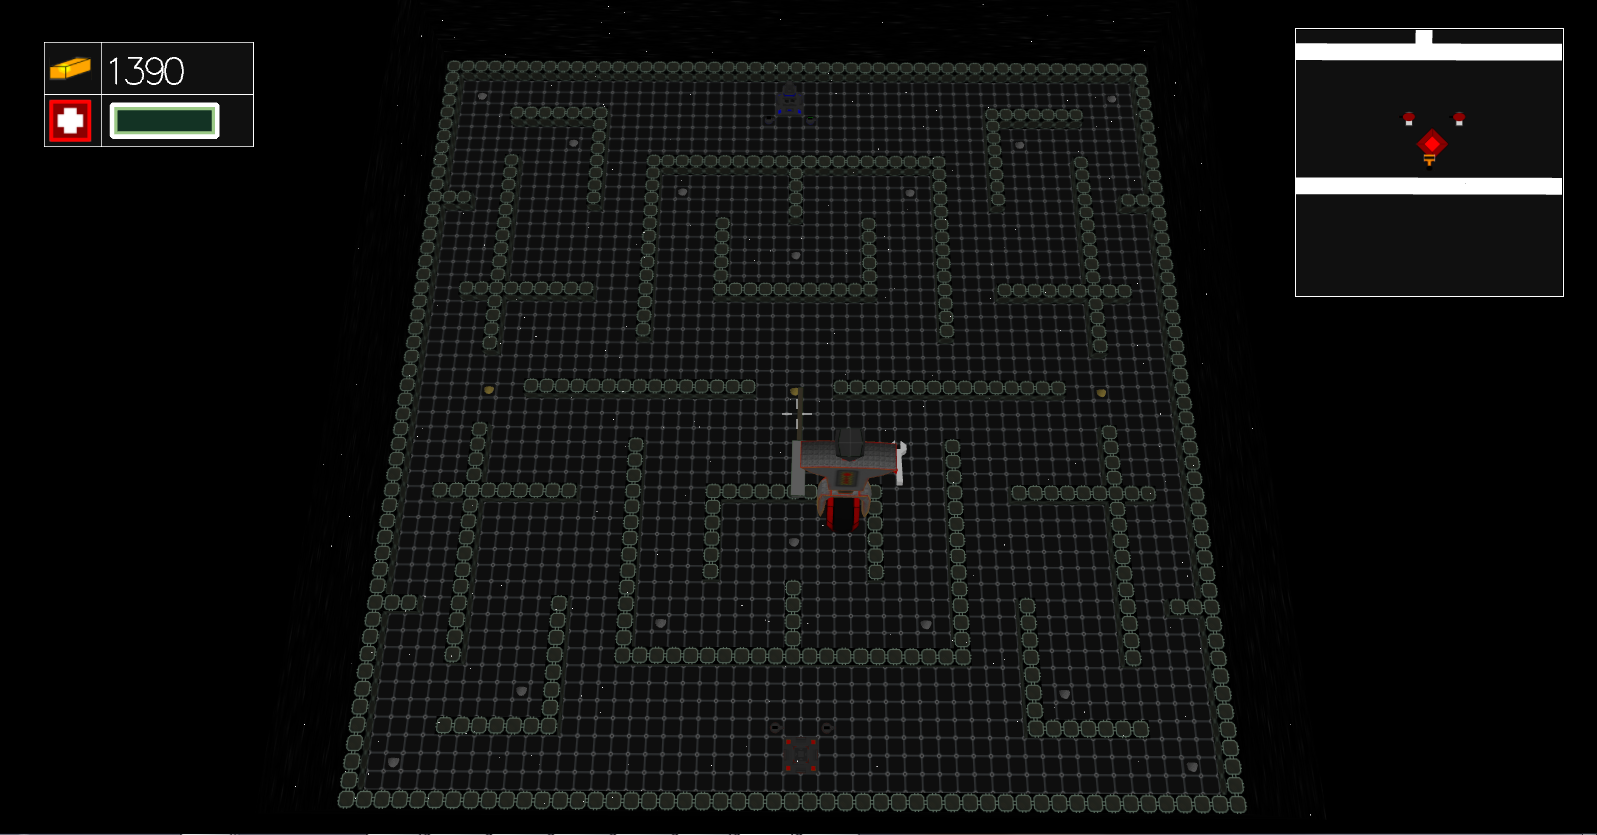
\includegraphics[width=\textwidth]{kaart.png}
	\caption{Een bovenaanzicht van het spel}
    \label{fig:terrein}
    \end{figure}

    \subsection{Spelers}
    De verschillende robot-bendes zijn te onderscheiden door kleuren. Zo is er een team Rood en een team Blauw. Standaard zit je in team Rood. Dit kan als volgt worden aangepast. Druk eerst op \textsc{Enter} en typ \textsc{set team b} in kleine letters. Vanaf dat moment zit je standaard in team Blauw: dit zal in werking treden als je het spel opnieuw opstart. Dit kan weer worden teruggedraaid door \textsc{set team a}.

    Je ziet de wereld vanuit de positie van je robot. De kijkrichting kan in elke willekeurige richting worden aangepast. Je robot zal dan meedraaien met de kijkrichting. Als de robot naar voren beweegt, zal de robot geleidelijk naar de kijkrichting draaien. Bij het schieten zal de laserstraal altijd in de huidige kijkrichting worden afgevuurd. De laserstraal heeft echter maar een beperkt bereik.

    Elke robot heeft een harnas. Bij het begin van het spel heeft de robot nog een volledig harnas. Zodra de speler wordt geraakt, wordt de conditie van het harnas slechter. Hierbij is grote voorzichtigheid vereist: je kan namelijk ook het harnas van andere leden uit jouw bende beschadigen. Een robot gaat dood als zijn harnas kapot is. In dat geval zal hij na een bepaalde hoeveelheid tijd terugkeren bij het commandocentrum met een volledig harnas.

    Je kan op het grondvlak vooruit en achteruit bewegen met een vaste snelheid. Je kan draaien door de kijkrichting aan te passen. Hierbij moet je natuurlijk op de kaart blijven. Ook kan je niet door gebouwen lopen. Het is wel mogelijk dat spelers door elkaar lopen. Je bestuurt het spel vanuit een derde persoon perspectief. Dit betekent dat je het spel bekijkt vanaf een punt vlak achter de speler. Het is bovendien mogelijk om te wisselen naar een eerste persoon perspectief door te \emph{scrollen}.

    \subsection{Gebouwen}
    Er zijn drie soorten gebouwen: torens, mijnen en commandocentra. Het bouwen van een toren kost 200 eenheden aan goud. Torens schieten op spelers en gebouwen van de andere robot-bende in hun bereik. Merk op dat torens een groter bereik hebben dan je eigen robot. Torens kunnen overal worden geplaatst onder de voorwaarde dat er nog geen ander gebouw of delfplaats staat op die plek. Mijnen kunnen over delfplaatsen worden gebouwd met het doel de inkomsten van een team te vergroten.

    Er zijn twee typen deflplaatsen, normale en extra rijke delfplaatsen. Het bouwen van een mijn over een normale delfplaats kost 220 eenheden aan goud. Het bouwen van een mijn over een extra rijke delfplaats kost 320 eenheden aan goud. Een mijn, die over een normale delfplaats is geplaatst, levert periodiek 30 eenheden aan goud op. Een mijn, die over een extra rijke delfplaats is geplaatst, levert periodiek 60 eenheden aan goud op. Deze periode is gelijk voor beide delfplaatsen. Het veroveren van een extra rijke delfplaats kan dus van groot belang zijn om het spel te winnen.

    Het commandocentrum is het belangrijkste gebouw van een robot-bende: het levert bovendien periodiek 10 eenheden aan goud op. Als dit gebouw wordt vernietigd, heeft het bijbehorende team verloren. Gebouwen kunnen door spelers worden beschoten, waardoor deze worden beschadigd. Bij voldoende schade zal het gebouw worden vernietigd. Dan kan op deze plaats, indien gewenst, een ander gebouw worden geplaatst. Gebouwen kunnen ge\"identificeerd worden door de kleur van het gebouw, dat correspondeert met de kleur van het team.

    \subsection{Verzamelbare voorwerpen}
    Er is maar \'e\'en verzamelbaar voorwerp: een muntje. E\'en of meerdere muntjes worden achtergelaten door spelers die dood gaan en torens die worden vernietigd. Als een speler dood gaat, is de totale waarde van de muntjes gelijk aan de gezamenlijke kas van dat team gedeeld door twee keer het aantal spelers in het team. Als een gebouw wordt vernietigd, dan is de totale waarde van de muntjes gelijk aan de helft van de kosten voor dat gebouw.

    Een muntje is 20 eenheden in goud waard. Aangezien we natuurlijk altijd een geheel aantal muntjes achterlaten, zullen we indien nodig naar beneden afronden. Als een speler doodgaat, wordt bovendien nog de waarde van de muntjes afgetrokken van de gezamenlijke kas van die speler. Een muntje kan vervolgens opgepakt worden door alle spelers. De waarde van het muntje zal dan toegevoegd worden aan de kas van het bijbehorende team.

    \subsection{Initialisatie}
	Om het spel op te starten kan je simpelweg het spel openen. Dan zit je in een spel met \'e\'en speler, namelijk jezelf. Om een multiplayer spel op te starten heb je meerdere mogelijkheden, of je laat andere spelers met jezelf verbinden, of je verbind met andere spelers. Om met andere spelers te verbinden druk je de knop \textsc{Enter} in en typ je \textsc{Discover}. Op je scherm staan nu alle spelers die in hetzelfde subnet zitten als jezelf. 
	
	Je kan nu aan het spel meedoen door het nummer van \'e\'en van deze spelers te onthouden. Dit nummer staat voor de speler. Druk nu weer op de knop {Enter} en typ in \textsc{Join} gevolgd door een spatie en het nummer van een speler. Nu kan je meedoen aan hetzelfde spel als die speler.
	
    Bij de start van het spel staan alle spelers bij het commandocentrum. Zoals al eerder gezegd, hebben alle spelers dan nog een volledig harnas. Bovendien zit er dan voor 200 eenheden aan goud in de kas.

    \FloatBarrier

    \subsection{Besturing}
    \label{sec:UI}

    Naast het spel kan je het volgende op je scherm zien:
    \begin{itemize}
    \item De hoeveelheid goud van het team, deze hoeveelheid staat achter een goudstaaf.
    \item De sterkte van het harnas, die wordt weergegeven door middel van een statusbalk.
    \item Het vizier van de speler.
    \item Een plattegrond.
    \end{itemize}

    Je vizier wordt altijd in het midden van het scherm geplaatst. Het mikken met het vizier gebeurt dus door het veranderen van de kijkrichting. De speler wordt altijd iets links van dit vizier getekend. Voor de duidelijkheid hebben wij hier ook een figuur van gemaakt, zie figuur \ref{fig:UI}.
    \begin{figure}
    \includegraphics[width=0.9\textwidth]{../Graphics/UI.eps}
    \caption{De gebruikersomgeving tijdens het spel}
    \label{fig:UI}
    \end{figure}
    De besturing van de robot kan met de \textsc{wasd}-toetsencombinatie of door gebruik te maken van de pijltjes-toetsen. Hiervoor geven we de volgende tabel:
    \begin{table}[H]
        \small
        \centering
        \begin{tabular}{| l | l |}
        \hline
        Knop & Reactie \\ \hline
        \textsc{w} of $\uparrow$ & De robot beweegt, indien mogelijk, vooruit naar de huidige kijkrichting toe \\ \hline
        \textsc{a} of $\leftarrow$ & De robot draait naar links \\ \hline
        \textsc{s} of $\downarrow$ & De robot beweegt, indien mogelijk, achteruit van de huidige kijkrichting af \\ \hline
        \textsc{d} of $\rightarrow$ & De robot draait naar rechts \\ \hline
        \end{tabular}
        \caption{Knoppen met bijbehorende reactie}
        \label{tab:planning}
    \end{table}

    Het is belangrijk om te beseffen dat \textsc{a} of \textsc{d} alleen de richting van de robot aanpassen. Je robot rijdt op een wiel, dus dit kan natuurlijk alleen als de robot al naar voren of naar achteren aan het bewegen is. De kijkrichting kan worden aangepast door gebruik te maken van de muis. Door de muis naar boven of naar beneden te bewegen, kijkt de speler verder omhoog of omlaag respectievelijk. Op analoge wijze kan de speler naar links of naar rechts draaien door respectievelijk de muis naar links of naar rechts te bewegen.

    De speler kan schieten door op de linkermuisknop te drukken. Merk op dat het vizier altijd in het midden van het scherm blijft. Hierdoor is een directe correspondentie tussen muis, vizier en kijkrichting. We tekenen daarom ook geen muis in het scherm. Deze kan worden losgekoppeld door op de rechtermuisknop te drukken. Chatten is in het spel mogelijk door \textsc{t} te drukken. De tekst kan vervolgens worden verstuurd door \textsc{Enter} te drukken.

    \subsection{Het neerzetten van gebouwen}
    Om een gebouw neer te zetten moet je eerst op de knop \textsc{b} drukken. Dan ga je in de zogenaamde \emph{bouw-modus}. Er wordt dan op de ondergrond een rooster getekend. Door middel van het vizier kan je een plek op het rooster aanwijzen. Je kan door te klikken dan de opdracht geven om het gebouw neer te laten zetten. Op dat moment wordt de bijbehorende hoeveelheid goud uit de gezamenlijke kas gehaald. Vervolgens zal het gebouw uit de grond verrijzen. Na het neerzetten van het gebouw blijf je in de bouw-modus. Door nogmaals op de knop \textsc{b} te drukken ga je weer uit de bouw-modus. Dit kan gezien worden in figuur \ref{fig:gebouw}.

    \begin{figure}
    \centering
    \includegraphics[width=\textwidth]{../Graphics/UI2.pdf}
    \caption{Een voorbeeld van het neerzetten van een gebouw in de gebruikersomgeving}
    \label{fig:gebouw}
    \end{figure} 
\end{document} 